
\begin{center}
\Huge
	Trigonometriske funktioner og integraler
\end{center}
\section*{Integraler med trigonometriske funktioner}
\stepcounter{section}

De trigonometriske funktioner $\sin$, $\cos$ og $\tan$ optræder ofte i forbindelse med integraler, men det er typisk noget rod at arbejde med grader i forbindelse med disse integraler. Det er derfor en fordel, at vi nu har radianer som vinkelenhed. 

Som sidst bliver enhedscirklen på Figur \ref{fig:enhed} samt Tabel \ref{tab:trig} brugbare. 

\begin{figure}[H]
	\centering
	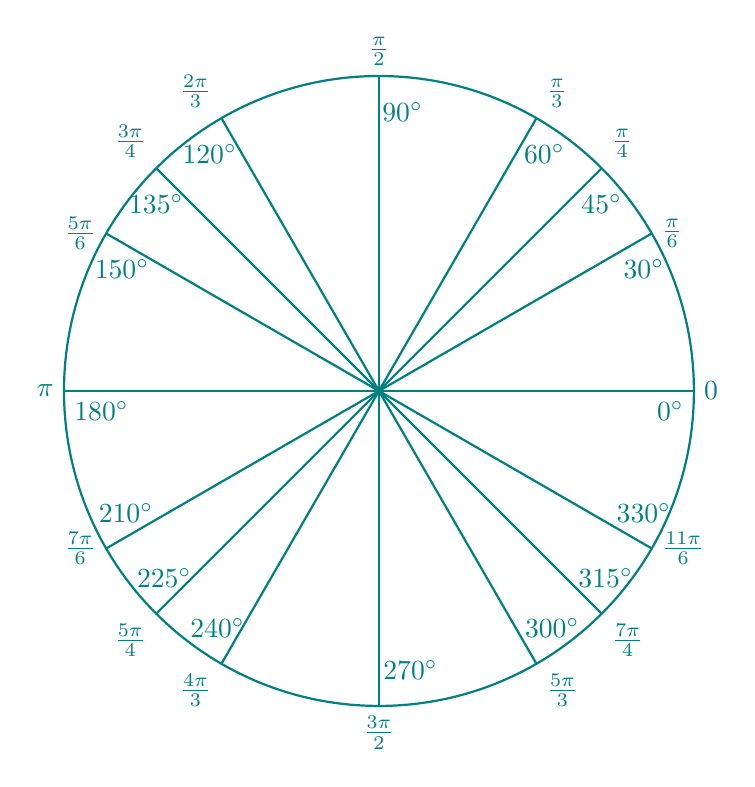
\begin{tikzpicture}
		\draw[thick, color = teal] (0,0) circle (4cm);
		\draw[thick, color = teal] (0,0) -- ({4*cos(0)},{4*sin(0)})
		node[pos = 1, anchor = north east] {$0^\circ$}
		node[pos = 1, anchor = west] {0};
		\draw[thick, color = teal] (0,0) -- ({4*cos(30)},{4*sin(30)})
		node[pos = 1, anchor = north, yshift = -0.2cm, xshift = -0.1cm] {$30^\circ$}
		node[pos = 1, anchor = west] {$\frac{\pi}{6}$};
		\draw[thick, color = teal] (0,0) -- ({4*cos(45)},{4*sin(45)})
		node[pos = 1, anchor = north, yshift = -0.2cm, xshift = -0cm] {$45^\circ$}
		node[pos = 1, anchor = south west] {$\frac{\pi}{4}$};
		\draw[thick, color = teal] (0,0) -- ({4*cos(60)},{4*sin(60)})
		node[pos = 1, anchor = north, yshift = -0.2cm, xshift = 0.1cm] {$60^\circ$}
		node[pos = 1, anchor = south west] {$\frac{\pi}{3}$};
		\draw[thick, color = teal] (0,0) -- ({4*cos(90)},{4*sin(90)})
		node[pos = 1, anchor = north, yshift = -0.2cm, xshift = 0.3cm] {$90^\circ$}
		node[pos = 1, anchor = south] {$\frac{\pi}{2}$};
		\draw[thick, color = teal] (0,0) -- ({4*cos(120)},{4*sin(120)})
		node[pos = 1, anchor = north, yshift = -0.2cm, xshift = -0.15cm] {$120^\circ$}
		node[pos = 1, anchor = south east] {$\frac{2\pi}{3}$};
		\draw[thick, color = teal] (0,0) -- ({4*cos(135)},{4*sin(135)})
		node[pos = 1, anchor = north, yshift = -0.2cm, xshift = -0cm] {$135^\circ$}
		node[pos = 1, anchor = south east] {$\frac{3\pi}{4}$};
		\draw[thick, color = teal] (0,0) -- ({4*cos(150)},{4*sin(150)})
		node[pos = 1, anchor = north, yshift = -0.2cm, xshift = 0.2cm] {$150^\circ$}
		node[pos = 1, anchor = east] {$\frac{5\pi}{6}$};
		\draw[thick, color = teal] (0,0) -- ({4*cos(180)},{4*sin(180)})
		node[pos = 1, anchor = north west] {$180^\circ$}
		node[pos = 1, anchor = east] {$\pi$};
		\draw[thick, color = teal] (0,0) -- ({4*cos(210)},{4*sin(210)})
		node[pos = 1, anchor = south, yshift = 0.2cm, xshift = 0.25cm] {$210^\circ$}
		node[pos = 1, anchor = east] {$\frac{7\pi}{6}$};
		\draw[thick, color = teal] (0,0) -- ({4*cos(225)},{4*sin(225)})
		node[pos = 1, anchor = south, yshift = 0.2cm, xshift = 0.1cm] {$225^\circ$}
		node[pos = 1, anchor = north east] {$\frac{5\pi}{4}$};
		\draw[thick, color = teal] (0,0) -- ({4*cos(240)},{4*sin(240)})
		node[pos = 1, anchor = south, yshift = 0.2cm, xshift = -0.05cm] {$240^\circ$}
		node[pos = 1, anchor = north east] {$\frac{4\pi}{3}$};
		\draw[thick, color = teal] (0,0) -- ({4*cos(270)},{4*sin(270)})
		node[pos = 1, anchor = south, yshift = 0.2cm, xshift = 0.4cm] {$270^\circ$}
		node[pos = 1, anchor = north] {$\frac{3\pi}{2}$};
		\draw[thick, color = teal] (0,0) -- ({4*cos(300)},{4*sin(300)})
		node[pos = 1, anchor = south, yshift = 0.2cm, xshift = 0.2cm] {$300^\circ$}
		node[pos = 1, anchor = north west] {$\frac{5\pi}{3}$};
		\draw[thick, color = teal] (0,0) -- ({4*cos(315)},{4*sin(315)})
		node[pos = 1, anchor = south, yshift = 0.2cm, xshift = 0.05cm] {$315^\circ$}
		node[pos = 1, anchor = north west] {$\frac{7\pi}{4}$};
		\draw[thick, color = teal] (0,0) -- ({4*cos(330)},{4*sin(330)})
		node[pos = 1, anchor = south, yshift = 0.2cm, xshift = -0.1cm] {$330^\circ$}
		node[pos = 1, anchor = west] {$\frac{11\pi}{6}$};
	\end{tikzpicture}
	\caption{Enhedscirklen med udvalgte vigtige vinkler.}
	\label{fig:enhed}
\end{figure}

\begin{table}[H]
	\centering
	\rowcolors{1}{SeaGreen!20}{Melon!20}
	\begin{tabular}{cccccc}
		$\theta$ & 0 & $\frac{\pi}{6}$ & $\frac{\pi}{4}$ & $\frac{\pi}{3}$ & $\frac{\pi}{2}$ \\
		$\cos(\theta)$ & 1 &  $\frac{\sqrt{3}}{2}$ & $\frac{\sqrt{2}}{2}$ & $\frac{1}{2}$ & 0 \\
		$\sin(\theta)$ & 0 & $\frac{1}{2}$ & $\frac{\sqrt{2}}{2}$ &  $\frac{\sqrt{3}}{2}$ & 1 \\
		$\tan(\theta)$ & 0 &  $\frac{\sqrt{3}}{3}$ & 1 & $\sqrt{3}$ & 
	\end{tabular}
	\caption{Vigtige funktionsværdier for cos, sin og tan.}
	\label{tab:trig}
\end{table}

Lad os betragte et eksempel.

\begin{exa}
	Vi får det bestemte integral
	\begin{align*}
		\int_0^{\frac{\pi}{2}} 2\cos(x) dx
	\end{align*}
	givet.
	Vi husker på, at integranten har $2\sin(x) + k$ som stamfunktion, og derfor får vi, at
	\begin{align*}
		\int_0^{\frac{\pi}{2}} 2\cos(x) dx &= \big[2\sin(x)\big]_0^{\frac{\pi}{2}} \\
		&= 2\sin\left(\frac{\pi}{2}\right) - 2\sin(0) \\
		&= 2 \cdot 1 - 2 \cdot 0 \\
		&= 2.
	\end{align*}
\end{exa}
Vi kan også støde ind i lidt mere komplicerede integraler.
\begin{exa}
	Vi betragter det bestemte integral
	\begin{align*}
		\int_{\frac{\sqrt{\pi}}{2}}^{\sqrt{\pi}} 2x\sin(x^2) dx.
	\end{align*}
	Vi husker på, at denne type integraler kan løses ved integration ved substitution. Vi lader $u = x^2$ og får
	\begin{align*}
		du = 2x dx \Leftrightarrow dx = \frac{du}{2x}.
	\end{align*}
	Vi laver nu substitutionen og finder det ubestemte integral med $u$ som variabel. 
	\begin{align*}
		\int 2x\sin(x^2) dx &= \int 2x\sin(u) \frac{du}{2x} \\
		&= \int \sin(u) du \\
		&= -\cos(u) + k \\
		&= -\cos(x^2) + k.
	\end{align*}
	Vi bruger nu denne stamfunktion for finde det bestemte integral.
	\begin{align*}
		\int_{\frac{\sqrt{\pi}}{2}}^{\sqrt{\pi}} 2x\sin(x^2) dx &= \Big[-\cos(x^2)\Big]_{\frac{\sqrt{\pi}}{2}}^{\sqrt{\pi}} \\
		&= -\cos\left(\left(\sqrt{\pi}\right)^2\right) + \cos\left(\left(\frac{\sqrt{\pi}}{2}\right)^2\right) \\
		&= -\cos(\pi) + \cos\left(\frac{\pi}{4}\right) \\
		&= 1 + \frac{\sqrt{2}}{2}
	\end{align*}
\end{exa}

\subsection*{Opgave 1}
Udregn følgende ubestemte integraler
\begin{align*}
	&1) \  \int 2\sin(x) dx   &&2) \  \int 3\cos(x) dx  \\
	&3) \  \int 4\sin(2\theta) d\theta   &&4) \   \int 6\cos(3x) dx   
\end{align*}

\subsection*{Opgave 2}
Find værdien af følgende bestemte integraler
\begin{align*}
	&1) \  \int_0^{\pi}	4\sin(x) dx   &&2) \  \int_0^{\frac{\pi}{2}} 3\cos(x) dx  \\
	&3) \  \int_{\frac{\pi}{3}}^{\frac{2\pi}{3}} 2\sin(2x) dx  
\end{align*}

\subsection*{Opgave 3}
Find følgende ubestemte integraler ved hjælp af integration ved substitution.
\begin{align*}
	&1) \ \int 9x^2\cos(x^3) dx   &&2) \  \int \sin(\theta)e^{2\cos(\theta) + 1} d\theta  \\
\end{align*}

\subsection*{Opgave 4}

Find værdien af følgende bestemte integraler ved hjælp af integration ved substitution.
\begin{align*}
	&1) \  \int_0^{\frac{\pi}{2}} \sin(x)^3\cos(x) dx   &&2) \  \int_{0}^{\pi} \frac{\cos(x)}{1 + \sin(x)} dx  \\
\end{align*}

\subsection*{Opgave 5 (Med hjælpemidler)}

Vandstanden i Ribe kammersluse kan den 1. marts 2026 beskrives ved funktionen 
\begin{align*}
	h(t) = 0.61\sin(0.48t + 1.35) + 0.98
\end{align*}
hvor $h(t)$ er vandstanden i meter over LAT (Laveste Astronomiske Tidevand) og $t$ er den forløbne tid i timer efter midnat.

\begin{enumerate}[label = \roman*)]
	\item Tegn grafen for $h(t)$ for $0 \leq t \leq 24$.
	\item Bestem den maksimale vandstand i Ribe kammersluse den 1. marts 2026.
	\item Afgør, hvor lang tid der går mellem to højvande den 1. marts 2026.
	\item Bestem den gennemsnitlige vandstand i Ribe kammersluse den 1. marts 2026.
\end{enumerate}

\subsection*{Opgave 6}
Integraler er ofte en besværlig størrelse at løse, og derfor er det en fordel at have flere værktøjet i sin værktøjskasse. Et af disse kaldes delvis (partiel) integration og tilsvarer i sin essens produktreglen for differentiation på samme måde som integration ved substitution tilsvarer kædereglen for differentiation. Vi har følgende formel for delvis integration:
\begin{align*}
	\int f'(x)g(x) dx = f(x)g(x) - \int f(x)g'(x) dx
\end{align*}

Anvend delvis integration til at bestemme følgende integraler. 
\begin{align*}
	&1) \  \int x\sin(x) dx   &&2) \  \int x^2\cos(x) dx  \\
\end{align*}
